\documentclass[10pt, letterpaper]{article}
\usepackage[cm]{fullpage}
\usepackage{algpseudocode}
\usepackage{algorithm}
\usepackage{graphicx}
\usepackage[section]{placeins}
\usepackage[table]{xcolor}

\algrenewcommand\Return{\State \algorithmicreturn{} }%


\title{Largest Subarray}
\author{Daiwei Chen \and Joseph Watts}

\begin{document}
	\maketitle
	\begin{abstract}

	\end{abstract}
	\section{Background and Related Work}

	\subsection{Brute Force Algorithm}

	\begin{algorithm}
	\begin{algorithmic}
		\caption{Brute Force}\label{bruteforce}
	\Function{bruteForce}{A}
	\State $n\gets len(A)$
	\State $maxsum\gets A[0]$
	\For{$i$ in 0..$n$-1}
	\For{$j$ in $i$..$n$-1}
	\State $total\gets 0$
	\For{$k$ in $i$..$j$}
	\State $total\gets total + A[k]$
	\EndFor
	\If{$maxsum < total$}
	\State $maxsum\gets total$
	\EndIf
	\EndFor
	\EndFor
	\EndFunction
	\end{algorithmic}
	\end{algorithm}

	This brute force algorithm will solve the problem of finding the largest sum of a subset of an array.
	The algorithm works by keeping track of two main index values.
	The first index is for the outer loop which will run between 0 and the number of elements in the array, while the second keeps track of the ending index and runs between the starting index and the number of elements in the array.
	This will allow for the capture of every possible subset of the array.
	The second index will contain a value between the first index value used by the outer loop and the number of elements in the array.
	A value to keep track of the sum of our array is made and then the array is summed between the two indexes.
	If our summed value is higher than our highest previously summed value, then update it to the new value.
	At this point the second index will be incremented, causing the sum between the indexes to take place again.


	% Explanation of runtime complexity
	Due to these three nested summations, the brute force algorithm runs in $O(n^3)$ time.
	The inner index loops all the way through the array, which means there will be $n$ iterations.
	The second loop changes the ending index inside of the previous loop from the starting index until the end of the array leading to an $O(n^2)$ algorithm.
	The range between the two indexes is then looped through again, causing the algorithm to become $O(n^3)$.
	It should be noted, however, that there is a slightly different version of this brute force algorithm that runs in $O(n^2)$ time by doing the sum as part of the second loop.
	
	This algorithm can be written as a summation where $i$ is the starting index, $j$ is the ending index, $k$ is the index for the loop doing the summing between $i$ and $j$, and $n$ is the number of elements in the array.
	% Summation Equation
	\[\sum_{i = 0}^{n-1}\sum_{j = i}^{n-1}\sum_{k = i}^{j}1\]
	
	\subsection{Kadane Algorithm}

  \begin{algorithm}
		\caption{Merge Sort}\label{mergesort}
	\begin{algorithmic}
	\Function{MergeSort}{L}
	\If{$len(L) <= 1$}
	\Return {L}
	\EndIf
	\State $A\gets$\Call{MergeSort}{first half of L}
	\State $B\gets$\Call{MergeSort}{second half of L}\\
	\Return {\Call{Merge}{A,B}}
	\EndFunction
	\end{algorithmic}
	\end{algorithm}

  Explain Kadane Here
  \[
	\textnormal{Gimme big O calculation pls}
	\]
	Explain big O and big $\Theta$ here
	\section{Experimental Setup}
	RUST HAS BIG PP OWO

	This is how we timed our setup
	\section{Results}
	Include our graph visualization of our data here. Brute Force and Kadane Timing
	

	% Add the graph showing the time taken.
	\begin{figure}[!htb]
	\center{
		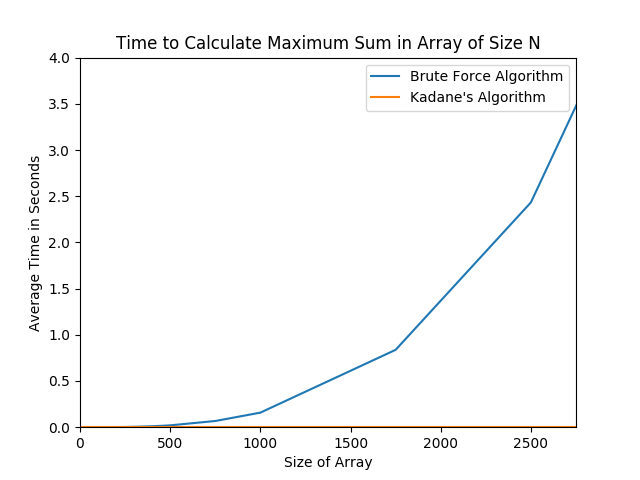
\includegraphics[width=0.75\textwidth] {python/avgTimeGraph.png}
	}
	\caption{
		\label{fig:time-graph} Graph of Brute Force vs Kadane Timings
	}
	\end{figure}

	% Add a table showing the time taken.
	
	\begin{figure}[!htb]
	\begin{center}
	\caption{
		\label{fig:time-table} Table of Brute Force vs Kadane Timings
	}
	\medskip
	\begin{tabular}{ | p{2cm} | l | l | }
			\hline
			Size of Array & Brute Force (s) & Kadane (s) \\ \hline
			1 & 0.000000033 & 0.000000025 \\ \hline
			5 & 0.000000085 & 0.000000036 \\ \hline
			10 & 0.000000448 & 0.000000051 \\ \hline
			50 & 0.000030930 & 0.000000125 \\ \hline
			100 & 0.000194367 & 0.000000184 \\ \hline
			150 & 0.000594095 & 0.000000260 \\ \hline
			200 & 0.001366055 & 0.000000331 \\ \hline
			250 & 0.002607847 & 0.000000402 \\ \hline
			300 & 0.004420136 & 0.000000466 \\ \hline
			350 & 0.006950275 & 0.000000573 \\ \hline
			400 & 0.010421218 & 0.000000639 \\ \hline
			450 & 0.014655456 & 0.000000716 \\ \hline
			500 & 0.020030729 & 0.000000956 \\ \hline
			750 & 0.067125954 & 0.000001231 \\ \hline
			1000 & 0.157617270 & 0.000001779 \\ \hline
			1750 & 0.837418008 & 0.000002682 \\ \hline
			2500 & 2.432867191 & 0.000003601 \\ \hline
			3500 & 6.606255604 & 0.000005064 \\ \hline
		\end{tabular}
	\end{center}
\end{figure}
	\section{Conclusions}
	As cleary shown through our graph and time table found in section 3,
	Kadane's algorithm is a much more optimized solution to solve the problem of finding the maximum sum of values within an array. 
	A brute forcing algorithm can be simplified down to $O(n^2)$, but our algorithm runs in $O(n^3)$.
	At the same time Kadane's algorithm runs in $O(n)$ time meaning that it will execute much faster.
	The amount of time that this algorithm saves is exponential.
	\end{document}
